
For the working mathematician, a basic application goes something like this.  The Fibonacci sequence $F_n$ ($n= 1, 2, \ldots$) is a \textit{strong divisibility sequence}, in that we have $\gcd(F_n, F_m) = F_{\gcd(n,m)}$; in particular, $F_m$ divides $F_n$ if $m \, | \, n$.  This fact was used by \'Edouard Lucas for Mersenne prime testing.  What about the special case $F_{3n}/F_n$?  And how could one possibly investigate this question using Gr\"obner bases?  It turns out that there is an identity:
\begin{equation}\label{F3n}
(F_{3n} - 5 F_n^3 - 3 F_n)(F_{3n} - 5 F_n^3 + 3 F_n) = 0,
\end{equation}
which explains explicitly this strong divisibility in this case.  How was such an identity obtained?  Here is the code:
\begin{M2}
\begin{verbatim}
i1:  R = QQ[z, x, y, t, MonomialOrder => Eliminate 2]
i2: I = ideal(x + y - z, (x*z - y^2)^2 - 1, t - z^3 - y^3 + x^3)
i3: toString groebnerBasis I
o3 = matrix {{25*y^6-10*y^3*t-9*y^2+t^2, z-x-y, ...
\end{verbatim}
\end{M2}  
\medskip
The variables $z,x,y,t$ represent $F_{n+1}, F_{n-1}, F_n, F_{3n}$, respectively.  The first polynomial defines the recurrence, the second is Cassini's identity, and the third is Lucas's identity.

One can check that factoring the first polynomial in the list above gives (\ref{F3n}).  Bootstrapping this with extra equations, we can discover that:
\begin{equation}\label{F5n}
(F_{5n} - 25 F_n^5 - 25 F_n^3 - 5 F_n)(F_{5n} - 25 F_n^5 + 25 F_n^3 - 5 F_n) = 0,
\end{equation}
In turn, this incites conjectures and proofs.  
For instance, we leave it to the reader to use modular arithmetic to verify from (\ref{F5n}) that the integer $\frac{F_{5n}}{5F_n}$ always has unit digit $1$.  This is an example of the promise of symbolic computation (with Gr\"obner bases) for the recreational mathematician, but there is more than this possible.

If you are dealing with an interesting problem, it is likely NP-hard.  Thus, any method that can cut down on the exponential search space and finish in a reasonable amount of time is a success.  

Consider the case of vertex 3-colorings of graphs.  Although exponential in the worst-case \cite[pp. 400]{yap2000fundamental}, Gr\"obner bases methods can be used to check or disprove conjectures in graph theory.  This was outlined theoretically in \cite{bayer1982division}, with success on a moderate-sized example \cite{hillar2008algebraic}, so-called Xu's conjecture \cite{shaoji1990size}, previously proved by other means and in much greater generality \cite{akbari2001kr}.

\begin{figure}
\begin{center}
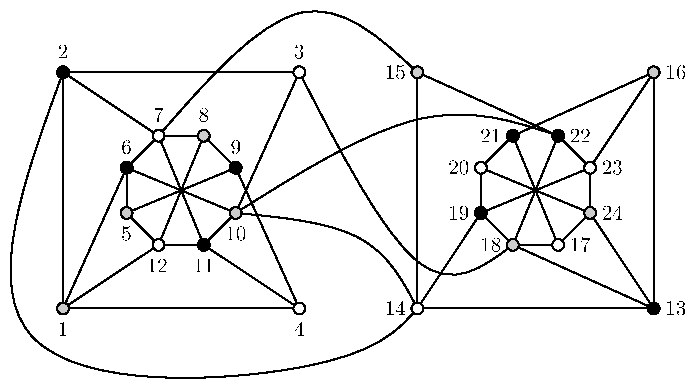
\includegraphics[width=.8 \linewidth]{akbarigraph.pdf}
\caption{Uniquely vertex 3-colorable graph without triangles: a counterexample \cite{akbari2001kr} to Xu's conjecture \cite{shaoji1990size}, which can be proved using Gr\"obner bases \cite{hillar2008algebraic}.}\label{graph}
\end{center}
\end{figure}

But all of this is classical.  What we are interested in are questions where there are not four or even twenty-four indeterminates, but rather an infinite number of them.  Take for instance, the following basic question about ideal membership.  

Setup problem in terms of ideal membership up to symmetry.  
%Note that might need arbitrarily large numbers of generators \cite{hillar2008minimal}.  

Developing the machinery to solve such questions is more than an intellectual curiosity.  Basic facts can now be proved by computer such as Theorem \ref{toric2x2}, but also cutting edge conjectures can be answered using these methods.  For instance, using \cite{EquivariantGB}, it is possible to verify the first non-trivial case of a basic finiteness conjecture for toric ideals \cite{draisma2013noetherianity}.  

\begin{theorem}\label{monomthm}[Proved by computer]
For $n > 1$, let $I_n = \ker (y_{ij} \mapsto x_i^2 x_j)$, $1 \leq i \neq j \leq n$.  The invariant chain of toric ideals $I_2 \subset I_3 \subset \cdots$ stabilizes up to the symmetric group.  That is, there is some $N$ such that all elements of $I_m$, $m > N$, are polynomial consequences of relabellings of a finite set of generators of $I_N$.
\end{theorem}

%We note that whether there is always an equivariant Gr\"obner bases is still an open question.

We next list the various applications of computation in rings with infinite numbers of indeterminates.  
We stick to applications algebraic in nature although there are interesting topological directions (e.g., Homological stability \cite{randal2013homological, church2012homological}).


\subsubsection{Group theory and Chemistry}

The first use of finite up to symmetry for polynomial ideas that we are aware of is in the group theory work of Cohen in \cite{cohen1967laws}.  
Independently, it was problems in algebraic chemistry \cite{ruch1967vandermondesche}, brought to the attention of the authors of \cite{aschenbrenner2007finite} by Andreas Dress, that inspired further applications of asymptotic polynomial algebra in chemistry \cite{Draisma08b}.

\subsubsection{Algebraic Statistics}

One of the major motivations for EGBs and infinite symbolic algebra is the the field of algebraic statistics.  One such application is to the problem of sampling from conditional distributions by algebraic methods \cite{diaconis1998algebraic}.  At its essence, the strategy is to find a set of moves through model space that preserves the sufficient statistics of the data.   The idea now is to consider growing families of model classes and show that up to obvious symmetries only a finite set of moves suffices for all infinite numbers of models (e.g., \cite{aoki2003minimal, santos2003higher, hocsten2007finiteness, drton2007algebraic, Draisma08b, Brouwer09e, draisma2009ideals, hillar2012finite, draisma2015finiteness}).

\subsubsection{Algebraic Geometry}

There are many natural situations in which finiteness up to symmetry and EGBs play important roles.  For instance, this occurs when studying the moduli space $n$ points in a line \cite{howard2009equations}, Betti tables as their length goes to infinity \cite{ein2015asymptotics}, geometry as the positivity of the the embedding line bundle grows \cite{ein2012asymptotic}, and limiting Grassmanians \cite{draisma2015plucker}.  The study of tensor geometry has also led to many practical successes.  One notable result is that bounded border rank tensors are cut out by equations in bounded degree \cite{draisma2014bounded} (independent of the size of the tensor).

%\subsubsection{Topology}
%
%Often, one encounters .

\subsubsection{Toric Algebra}

Much of the inspiration for asymptotic polynomial algebra comes from the study of certain chains of toric ideals, many of which arise naturally in algebraic statistics.  The series of works \cite{Hillar13, hillar2016corrigendum, draisma2013noetherianity, KKL:equivariant-markov} has developed fundamental finiteness properties of these structures.  Basic questions remain open, however, as we outline in Section \ref{sec:challenges}.

\subsubsection{Representation and category theory}

The theory of FI-algebras \cite{church2014fi, church2015fi} has been developed recently with the symmetric group a central object.  In this regard, we have equivariant Hilbert series \cite{Nagel}, \cite{krone2016hilbert} in the commutative algebra of invariant ideals \cite{hillar2012finite}. In the direction of different groups other than the symmetric group, there has bee work on the general linear group \cite{putman2014representation, sam2016gl}.  More recently, Gr\"obner methods have been used to understand  representations of combinatorial categories \cite{sam2016grobner}.




